%%---------------Appendices--------------------------------
\appendix
\chapter{this is Appendix A}
% In order to mimic the data coming from an infinite stream, it was necessary to convert the limited duration into a data stream. The data stream simulation tools are described next, followed by the description of the use cases.


% \section{Data Stream Simulation}
% Since data used in this research were obtained from concluded experiments, it was essential to find a mechanism to convert the batches of data in to a data stream. The streaming data was generated from the target datasets by applying the Scikit-Multiflow package in Python for the DSAP algorithm and the DSD objects in the stream package in R for the streaming K-means algorithm. 



% \subsection{Scikit-Multiflow-based Simulation}
% The 'scikit-multiflow' framework in Python programming language is a free and open-source tool for generating data stream \cite{montiel2018scikit}. It provides multiple stream learning methods, steam generators, and evaluators, where the primary focus is on batch learning. This framework's base class is the 'StreamModel', which has abstract methods to be implemented by classes. A 'StreamModel' object interacts with other objects: ' Stream' and 'StreamEvaluator'. The 'stream' gives an endless flow of data by request, and 'StreamEvaluator' presents various tasks that are queries the stream, train, test on the incoming data, and tracks the model's performance.

% 'scikit-multiflow' needs NumPy library installed in the system. All classes are shown in Figure \ref{sci} for generating data stream. The \textit{skmultiflow} data contains data stream methods, including methods for batch-to-stream conversion and generators. In all classes, the stream is available upon request and old data points cannot be accessed at a later time. These are listed below:

% %\renewcommand\labelitemi{$\vcenter{\hbox{\tiny$\bullet$}}$}
% \begin{itemize}
%     \item {data.base\_stream.Stream:} it defines the minimum requirements of a stream and it can work along with other modules in multiflow. 
%     \item {data.DataStream:} it takes the whole data consisting of the $X$ as features and $Y$ as targets or takes them separately.
%     \item {data.FileStream:} if the data previously collected and stored in the CSV file (it just supports CSV files at this moment), it can generate streams by loading the dataset. 
%     \item {data.ConceptDriftStream:} this stream generator adds concept drift by joining several streams and giving the weight. 
%     \item {data.TemporalDataStream:} takes the dataset containing $X$ as a features and $Y$ as a targets with $time$ as a timestamps. 
% \end{itemize}

% On the other hands, as shown in Figure \ref{sci}, there are many stream generators classes for different problems listed below:
% %\renewcommand\labelitemi{$\vcenter{\hbox{\tiny$\bullet$}}$}

% \begin{itemize}
%     \item[$-$]  data.WaveformGenerator: random differentiation of some base waveforms.
%     \item[$-$]  data.SineGenerator: sine waves stream generator.
%     \item[$-$]  data.AgrawalGenerator: scaling up decision tree learners based on Agrawal model.
%     \item[$-$]  data.AnomalySineGenerator: simulate a stream with anomalies in sine waves.
%     \item[$-$]  data.LEDGenerator: seven-segment LED display stream generator.
%     \item[$-$]  data.LEDGeneratorDrift: add concept drift to the LED stream.
%     \item[$-$]  data.MixedGenerator:  data stream with abrupt concept drift and boolean noise-free.
%     \item[$-$]  data.MultilabelGenerator: the stream of samples for a multi-label problem.
%     \item[$-$]  data.RandomRBFGenerator: Random Radial Basis Function stream generator.
%     \item[$-$]  data.RandomTreeGenerator: based on a random tree that splits features at random and sets. 
%     \item[$-$]  data.RegressionGenerator: creates a regression stream.
% \end{itemize}


% \begin{figure}
% \centering
% 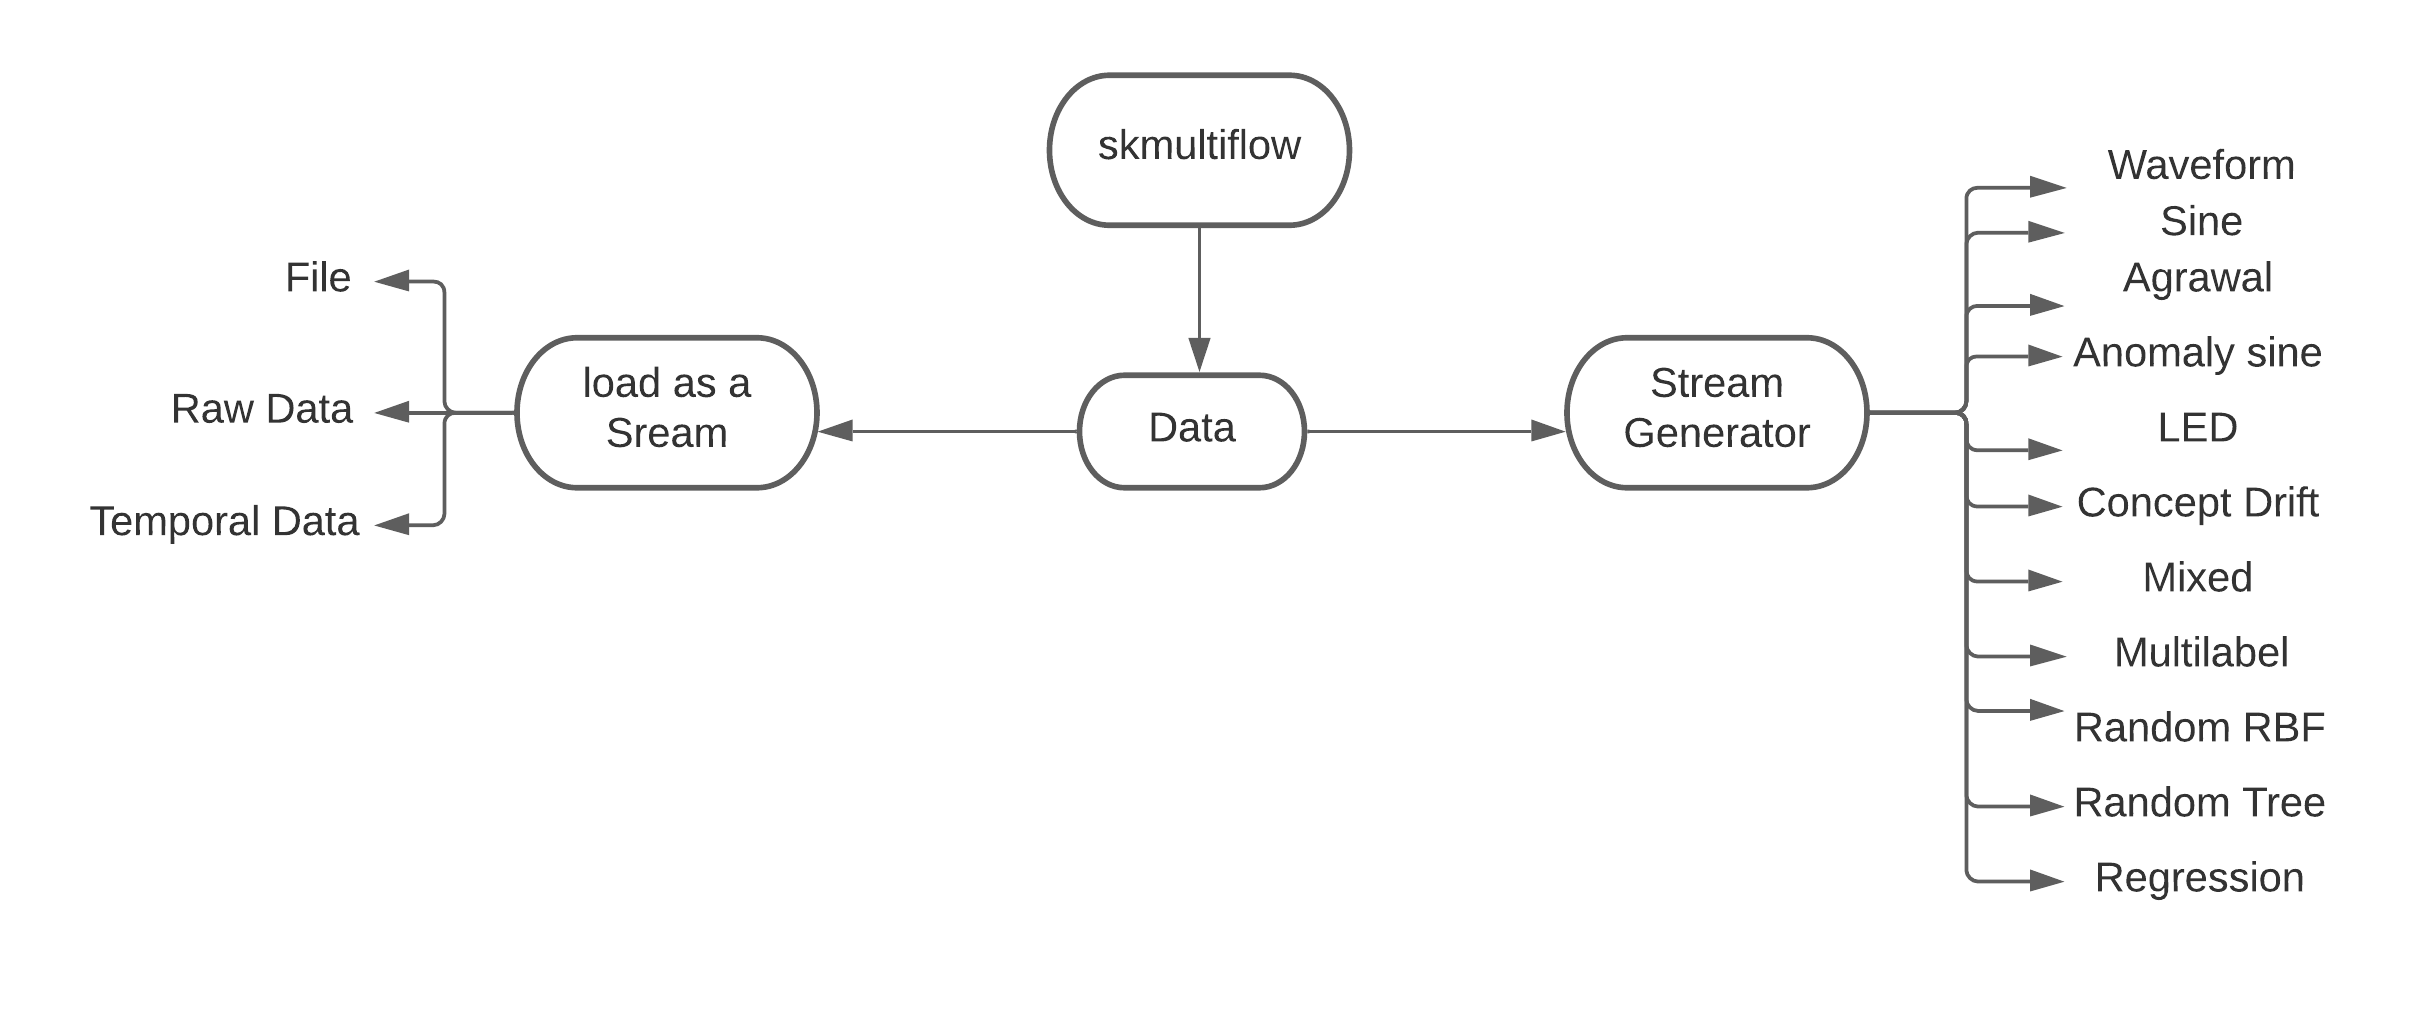
\includegraphics[width = 12cm,height = 6cm]{image/sci2.png}
% \caption{The scikit-multiflow map with multiple methods for generating data. }
% %\cite{SMF}}
% \label{sci}
% \end{figure}



% \subsection{DSD-based Simulation}
% Data Stream Data or DSD, part of 'stream' in R programming language, is a simulation package \cite{hahsler2017introduction} used for streaming K-means. This package can be a management layer or a wrapper for the stored data, or a generator that simulates a data stream with known features for controlled experiments. 

% Figure \ref{DSD} shows the DSD classes in a hierarchy UML relationship. All DSD classes extend the abstract from the base class, Data Stream Data in R or  DSD\_R. This package provides simulated streams in three different ways: static structure, concept drift, or connectors to real data and streams. The static structure is used for simulating the random Gaussian, bench, and noise data stream. The concept drift is applied to generate a specific complex of a data stream with this concept. Connectors to real data DSD object has three categories as explained below.

% \begin{itemize}
%     \item\textbf{DSD\_Memory:} It gives a streaming interface to the matrix, static data in memory, representing a fixed portion of a data stream. Also, DSD\_Memory can generate a copy of a part of another DSD object to be replayed in experiments many times.
    
%     \item\textbf{DSD\_ReadCSV:}  It reads data line by line from a file or a connection and makes it available in a streaming manner. Then, it enables a system to process data that is larger than the available memory. Connections to real data can be applied to read from real-time data streams.
    
%     \item\textbf{DSD\_ReadDB:} KINI presents an interface to result set from a SQL query to any other relational database.  These databases can use the DBI interface. 
% \end{itemize}

% All the DSD packages have the same interface using the two functions: a creator function whose outcome is not a dataset but an object describing the stream's properties and its current state, and a data generating function that is handled to get the next data point from them stream represented by object k.


% \begin{figure}
% \centering
% \includegraphics[width = 9cm,height = 8cm]{image/Blank diagram66.png}
%  \caption{Overview of the data stream Data (DSD) class structure.}
% \label{DSD}%\cite{hahsler2017introduction}
% \end{figure}


% Although the above two packages are very capable of mimicking the data observed in data stream, but the user must acknowledge the limitations of such techniques. The difference from the real data stream can result from many potential shortcomings of the stream simulation models. The stream simulation packages do not have the support for generating realistic latency information, missing data, mixed timestamps, varying data cadence, and others. Hence any verification of the robustness and efficacy or benchmarking of a stream clustering algorithm done using the simulated streams should be cautiously accepted. The next sections show the details of the implementation of workflow phases explained earlier with the two positioning and occupancy datasets. 



%%%%%%%%%%%%%%%%%%%%%%%%%%%%%%%%%%%%%%%%%%%%%%%%%%%%%%%%%%%%%%%%%%%%%%%%%%%%%%%%%%%%%%%%%%%%%%%%%%%%%%%%%%%%%%%

% \subsection{LBAP :DSAP V.1.0}
% The DSAP version 1.0 is an extended AP clustering algorithm, that is capable of handling the sequence of the data in online and offline mode. Before that, AP could not handle our datasets because it is suffering from high memory consumption. DSAP version 1 is based on online Micro and offline Macro clustering as illustrated in framework \ref{frame1}.

% \begin{figure}
% \centering
% 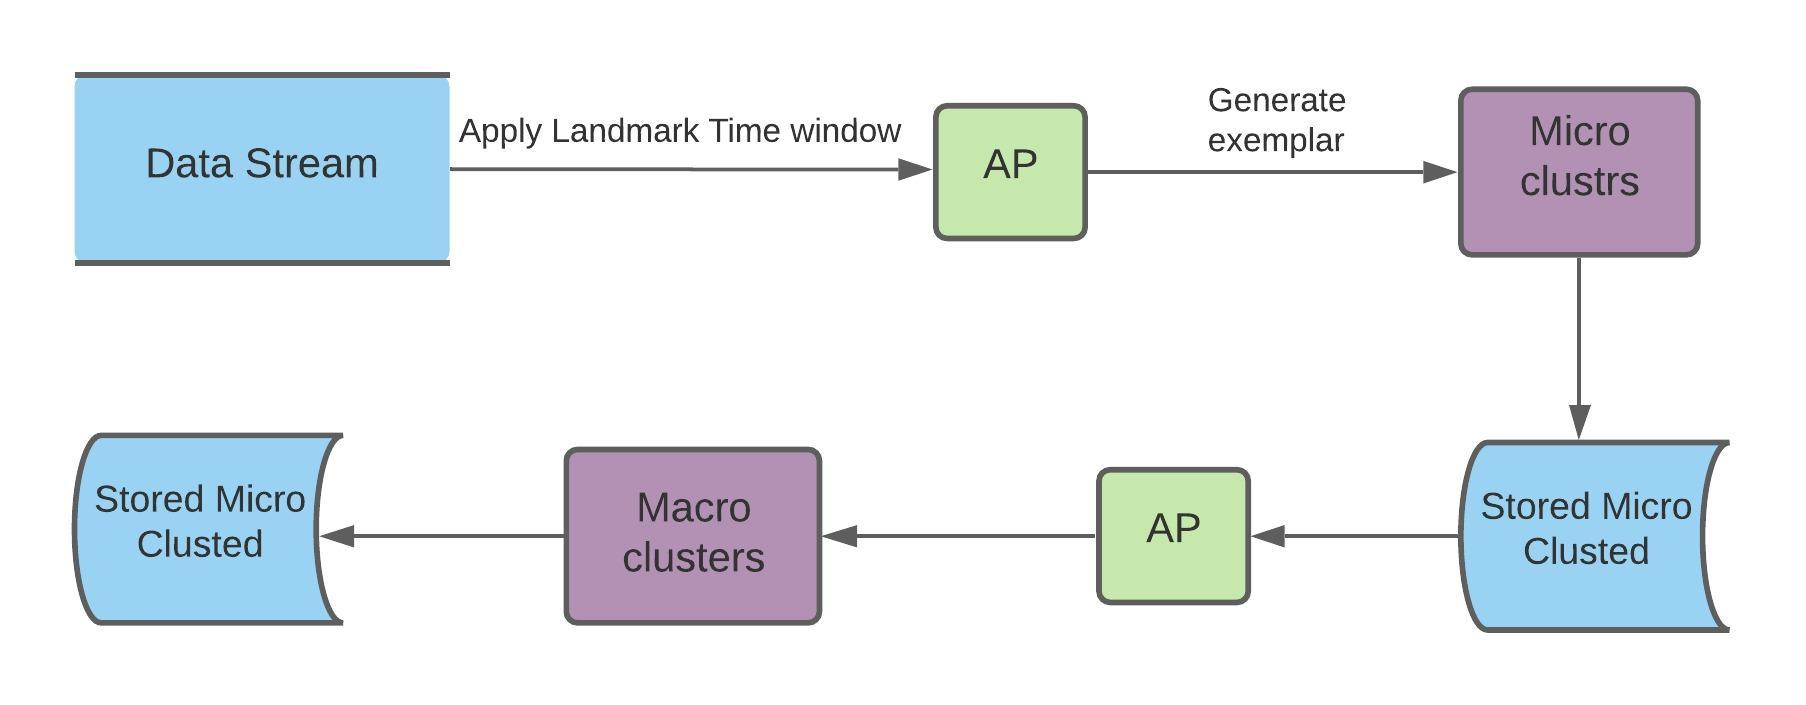
\includegraphics[width = 15cm,height = 7cm]{image/Blank diagram2.jpeg}
% \caption{The framework of DSAP version 1.0 algorithm}
% \label{frame1}
% \end{figure}

% For data stream clustering, a landmark time window model on the affinity propagation algorithm was applied. Time window models are used to extract a subset from the data stream. 
% e-counter and WiFi fingerprinting indoor Stream data can be described as an infinite sequence of tuples such as follows:
    
% \[    \left [  T_{1} =\left ( E{1},N_{1},\sum_{1},t{1} \right )  \right ], \left [ T_{2} = \left ( E_{2},N_{2},\sum_{2},t{1} \right ) \right ],\]
% \[
% ...,\left [ T_{n} = \left ( E_{i},N_{i},\sum_{i},t{i} \right ) \right ] \] 
    
%  where $E_{i}$ s an exemplar ranges, $N_{i}$ number of points, $\sum_{i}$ is a sum of each data point and exemplar, and $t{i}$ is the last time to merge to exemplar.
% \subsubsection{Online Phase}
% During the online Micro clustering phase, the data is divided into hourly landmark windows $L_i$ and the AP algorithm is applied for each hour to compute centroids to encapsulate the data stream . Then we slide the time window one hour ahead and repeat the process for the entire period. 

% % \begin{figure}
% % \centering
% % 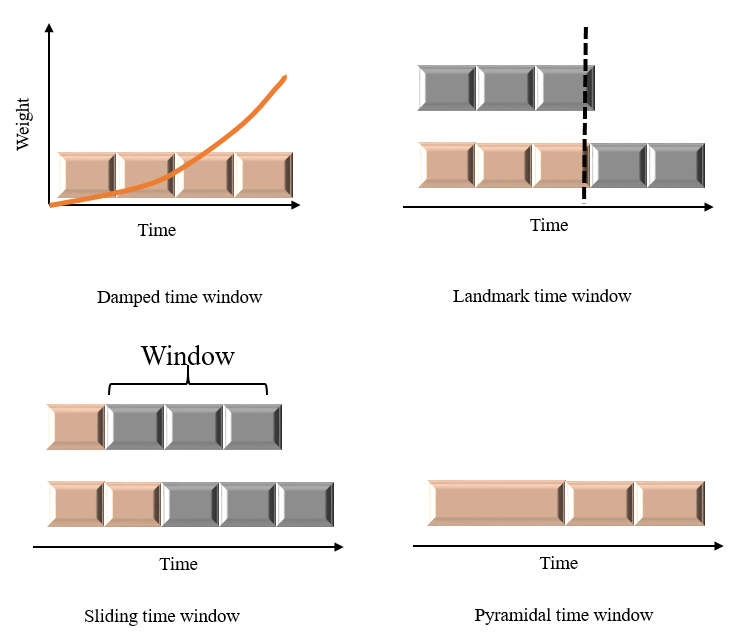
\includegraphics[width = 10cm,height = 4cm]{image/timeW.PNG}
% % \caption{1-Day Landmark time window model}
% % \label{timew}
% % \end{figure}

% \subsubsection{Offline Phase}
% At the end of each period, in the macro clustering, AP is again employed to generate the final clusters based on all the cluster centroids obtained from the micro-clustering phase.


%%%%%%%%%%%%%%%%%%%%%%%%%%%%%%%%%%%%%%%%%%%%%%%%%%%%%%%%%%%%%%%%%%%%%%%%%%%%%%%%%%
% \begin{algorithm}[H]
%     \SetKwInOut{Input}{Input}
%     \KwData{ Tuples: e-counter dataset $E=(E_{1}, E_{2},...,E_{n})$ for Micro clustering;  }
%     \textbf{Require for Micro and Macro:}
%     {, preference, Damping,  $max\_iter$}\newline
%         \textbf{Initialize:}\newline
%         Landmark time window (size $T_{s}$ = 60 minutes)\newline
%         Similarity Matrix: S $\forall$ i, k:  s(i, k) = 0\newline
%         {Availability Matrix: A $\forall$ i, k:  a(i, k)} = 0\newline
%         {Responsibility Matrix: R $\forall$ i, k:  r(i, k)} = 0\newline
%   	    \For {7a.m.  $\leq$ $T_{s}$ $\geq$ 7p.m.}{
%   	    \SetKwFunction{FIROC}{AP}
%         \SetKwProg{Fn}{Function}{:}{}
%         \Fn{\FIROC{E}}{
%   	    \emph{
%   	       \While{$r(i,k)$  $a(i,k) \neq$ convergence}{
%   	       $r(i, k) \leftarrow s(i, k) - \max\limits_{k' s.t. k' \neq k}\{ a(i, k') + s(i, k') \}$\newline
%   	       Availability A:\newline
%   	       $(i, k) \leftarrow \min\{0, r(k,k) + \sum\limits_{i' s.t. i' \notin \{i, k\}}{\max\{0, r(i',k)\}}$\newline
%   	       no-diagonal A:\newline
%   	       $a(i, k) \leftarrow \sum\limits_{i' \neq k}\max(0, r(i', k))$
%   	       }  	    }
  	       
%         }  	    \KwResult{Set of Tuples for Macro clustering:\newline $P=(P_1, P_2,...,P_n)$}
%     \SetKwFunction{FIROC}{AP}
%     \SetKwProg{Fn}{Function}{:}{}
%     \Fn{\FIROC{P}}{
%     \While{$r(i_1,k_1)$  $a(i_1,k_1) \neq$ convergence}{
%     $r(i_1, k_1) \leftarrow s(i_{1}, k_{1}) - \max\limits_{k'' s.t. k'' \neq k_{1}}\{ a(i_1, k'') + s(i_1, k'') \}$\newline
%     Availability A:\newline
%     $(i_1, k_1) \leftarrow \min\{0, r(k_1,k_1) + \sum\limits_{i'' s.t. i'' \notin \{i_1, k_1\}}{\max\{0, r(i'', k_1)\}}$\newline
% no-diagonal A:\newline
%   $a(i_{1}, k_{1}) \leftarrow \sum\limits_{i'' \neq k_1}\max(0, r(i'', k_1))$
%     }
%     }
%      \KwResult{Macro Clusters:\newline $C=(C_1, C_2,...,C_n)$} 
%         }
%   \caption{DSAP V.1.0 Algorithm}
%     \label{alg2}
% \end{algorithm}
%%%%%%%%%%%%%%%%%%%%%%%%%%%%%%%%%%%%%%%%%%%%%%%%%%%%%%%%%%%%%%%%%%%%%%%%%%%%%%%%